% Chapter Template

\chapter{Literature Review} % Main chapter title

\label{Chapter3} % Change X to a consecutive number; for referencing this chapter elsewhere, use \ref{ChapterX}

%----------------------------------------------------------------------------------------
%	SECTION 1
%----------------------------------------------------------------------------------------

\section{Introduction}
This section will go through the existing literature around the topic of GNSS spoofing and anti-spoofing. References were chosen based on their relevance in terms of
content as well as age. There have been some significant performance increases in technologies over the past 10 years.
This literature review will focus mainly on GNSS spoofing methods, with emphasis on the GPS constellation, and on potential anti-spoofing methods. While development of
anti-spoofing algorithms is not an aim of this thesis, knowledge of such methods allow for understanding potential attack vectors.

To ensure that the review of current literature is accurate, some exclusion criteria was implemented.

\begin{itemize}
    \item Exclusion criteria \\ To help narrow the scope of the literature review certain criteria was selected to be omitted
    \begin{itemize}
        \item Age of source: > 2010 for SDR specific | > 2008 for all others \\ When it comes to the implementation of spoofers using SDR platforms, the most up to date information is required since the software typically used in these cases are open source and prone to frequent changes.\\ This is less of an issue when detailing the operation of the GPS navigation system, or, to a lesser extent, effective spoofing attacks and defences. This is because most off the shelf receivers have not got any spoof mitigation built into their designs \cite{RN12}.
    \end{itemize}
    \item Inclusion criteria
    \begin{itemize}
        \item Application specifics \\ While not all sources will have an application, whether to attack or defend, it should be noted that there was an importance placed on getting sources that applied the theory described.
        \item SDR implementation \\ Since this project relied on the use of an SDR platform for the application of a spoofer it was important that a large number of sources also use a similar platform. This helped in forming a strategy to complete the project. It was also important so that time was not wasted reinventing the wheel.
    \end{itemize}
    \item Keywords
    \begin{itemize}
        \item GPS
        \item GPS Spoofing
        \item GNSS Spoofing defence
        \item GPS UAV Attack
        \item GPS Spoof mitigation
        \item GPS Spoofing autonomous vehicles
        \item meaconing
        \item GNSS threat analysis
        \item GNSS threat survey
    \end{itemize}
\end{itemize}

There was an exception to the age criteria \cite{RN11}. This was commonly referenced by many other sources so warranted inclusion. 

%----------------------------------------------------------------------------------------
%	SECTION 2
%----------------------------------------------------------------------------------------

\section{Literature Review}
How GPS works has been covered in depth over the past few decades. The operating principles for GPS and other GNSS systems is well known and was covered in the previous
chapter \ref{Chapter2}.

From literature the consensus is that the same thing that has made GPS ubiquitous with navigation and 
positioning has also made it a target for exploitation and manipulation. That is the workings
of the infrastructure are well known and public and are transparent and predictable \cite{RN7} \cite{RN4}. This is problematic since this infrastructure
is seen as a critical service by many industries including utility management, healthcare/ emergency services and security \cite{RN12} \cite{RN32}. \textcite{RN28} noted that the signals
presented to the receivers are usually trusted without any authentication or other checking. The authors show that this trust can be exploited without physical access to
or altering the software of the target device. One of the signal properties that makes spoofing simple is the received signal power from space which is less than -130dBm
making overpower the legitimate signal a simple task. Having such a system so prone to threats is not ideal. 

%
% Subsection - spoofing
%

\subsection{Spoofing Attack Literature} \label{Subsec:SpoofLit}
The further development of SDR platforms has driven down the cost of launching GNSS based spoofing attacks. Devices such as the Hack-RF, USRP, Blade-RF and others have
been documented for this use \cite{RN4} \cite{RN9}. These devices are all examples of Software defined radios that are capable of duplex operation. This combined with
open source software, as described in \cite{RN16} \cite{RN57} \cite{RN4}. The former is a software package, GPS-SDR, that converts a compatible SDR into a GPS receiver
without any knowledge of GPS or signal processing required. With some understanding this could be modified to capture the raw signal for use in a Meaconing spoofing
attack. The later refers to the setup and use of the GPS-SDR-SIM program. This program provides a method for producing a modulated GPS signal for transmission. It
requires the RINEX file for the date and time of the spoof attack as well as a set of coordinates to reproduce. Since it is open source it can be easily modified for any
use case. 

\textcite{RN28} created a spoofing device based on the HackRF SDR platform in conjunction with the open source program GPS-SIM-SDR. Hack-RF was chosen as the SDR platform
because of its open source nature, it also had the required specifications to perform the spoof attack. It was shown in this paper that the use of an SDR and open source
software was able to fool client devices such as apple smartphones into thinking they were else where. This included specific apps that require location data such as Uber
and DiDi. The authors provided a list of recommendations to minimise the risk of being spoofed. These recommendations are non trivial and some required alterations to how
the receiver processes the signal data.

\textcite{RN30} investigated the exact requirements for successfully spoofing a receiver. From the experiments it was found that there are 4 parameters that have required
values in order to successfully spoof a GPS signal. That is the relative signal power must be $\geq+2dB$, the constant time offset must be $\leq 75ns$, location offset
must be $\leq 500m$ and the relative time offset must be $\leq 80ns$. These values correspond to situations where the receiver already has a lock on satellites. It was
found that when values outside of those mentioned above, the lock would be lost and the spoofing would be unsuccessful. The more victims that are trying to be spoofed the
more restrictive the location for performing the spoof becomes.

Software based GPS simulation tools similar to that of GPS-SDR-SIM have also been created using a combination of C and MATLAB \cite{RN15}. In this example the author used
C to ensure processing efficiency of the modulated signal, and used MATLAB to simulate multi-path errors and uncertainty. The resultant file was then saved to the hard
drive of the host computer. This could then be loaded into an SDR for transmission, although this was not specifically touched on in the paper.

Over recent times there has been an increase in the industries that rely on the timing and positional data provided by GNSS systems. One such industry is autonomous
vehicles, in particular drones. Drones can be used for hobbies, professional photography/ videography or for surveillance purposes. They are small and can be controlled from great
distances. All commercially available drones have some form of GNSS/GPS location service built in, and as such they become a target for spoofing attacks. Some drone
manufactures have built in auto landing features in the event that the drone enters into restricted airspace's. This was to combat civilians who were flying within
airports, causing safety and security issues. This is one such way that spoofing attacks could be utilised now and in the future, by transmitting a signal that would make
the drone perceive itself to be in a restricted airspace and land. This kind of attack has been successfully conducted as shown in \cite{RN4}. 
\textcite{RN21} developed a system to perform a series of spoof attacks on UAVs based on an SDR \cite{RN23}. The goal of this was to be able to 
control the flight path of the UAV without raising any alarm's from the victim. This paper establishes the required conditions in which a UAV will
be susceptible to being captured from a spoofing attack, as well as the range of post capture control that the spoofer will have over the victim.
From testing it was found that spoof attacks were successful from up to 50m and up to a velocity of 10m/s.
Simulations were produced for analysis of post capture control of the UAV. 
When testing, both covert and overt spoofing methods were used, distinguished by whether or not the spoofer made an attempt to avoid detection. For the most part there
was no practical difference between covert and overt methods since the commercial GPS units did not trigger any anti spoof mechanism when being subjected to an overt
attack. Field testing showed that the spoof attempt caused unrecoverable navigation errors which resulted in the UAV crashing. Future work should increase the
sophistication of the attacks. This may decrease chances of the drone crashing due to unsuccessful attacks.

There has been research into ways that GPS spoofing attacks could be used in road navigation scenarios. \citeauthor{RN9} were able to implement an algorithm for road
network modelling and navigation spoofing using GPS. This algorithm coupled with a HackRF SDR meant that the authors were able to create a lunchbox sized spoofing device.
Although in research it was found that the victim devices were able to register a difference in location from network based sources and GNSS based sources, the victims
prioritised the location resolved from GNSS sources over network or cellular.
While this attack strategy may be successful against people not familiar with their surrounding area, someone who is familiar or is paying close attention should be able
to tell they are being led to an incorrect area. Where this is less likely to be the case is with driverless vehicles.
In the paper written by \citeauthor{RN25} \cite{RN25} regarding driverless vehicle safety, it was noted that there is a significant threat to these types
of systems that rely heavily on reliable GPS signals. Although there have been proposed solutions to this problem through the use of 
other sensor information available locally to each vehicle and in the form of an ad-hoc network known as V2V (vehicle to vehicle) and more broadly
V2X (vehicle to everything) \cite{RN17}, this is still in its infancy and will require joint work from all vehicle manufacturers. 

\citeauthor{RN12} commented on the effect of GNSS spoofing of a cooperative victim. That is when someone is willing to aid the attacker
in performing an attack. This may be implemented to circumvent position based restrictions or if being GPS tracked during certain activities.
\citeauthor{RN12} used the example of a fisherman wanting their GNSS receiver to falsely report the boat had stayed out of protected areas \cite{RN12}.

In \citeyear{RN6} \textcite{RN6} investigated the different spoofing and antispoofing techniques available. \citeauthor{RN6} noted that spoofing attacks can be divided into 3 main categories:
GPS signal simulator, Receiver-Based spoofers and Sophisticated Receiver based spoofers. These attack strategies come about because of vulnerabilities in the GPS system.
These vulnerabilities can be described in the three operational layers of GPS, signal processing, data bit, and position/navigation solutions.
Testing spoofing techniques is difficult to achieve since there are regulations around the emission of EM radiation at certain frequencies and power levels.
There were three methods used to test the spoofing/antispoofing techniques. These were Indoor re-transmissions, spoofing using recorded data (No RF transmission), and
using RF combiners to combine authentication and spoofed signals.
The results that were acquired showed that the commercial GPS receivers were vulnerable to a number of spoofing techniques.
Previous research into the effects of spoofing can be found in \cite{RN23}. This predates more modern methods for launching a successful spoofing attack and uses a
specialised DSP chip within a specialised hardware configuration. The findings of this paper was used to recommend anti-spoofing methods for unsophisticated spoofing
attacks. \citeauthor{RN23} was able to implement complex spoofing setups with multiple phase locked radios that were able to overcome some anti-spoofing techniques. 

\begin{figure}[h]
    \begin{centering}
        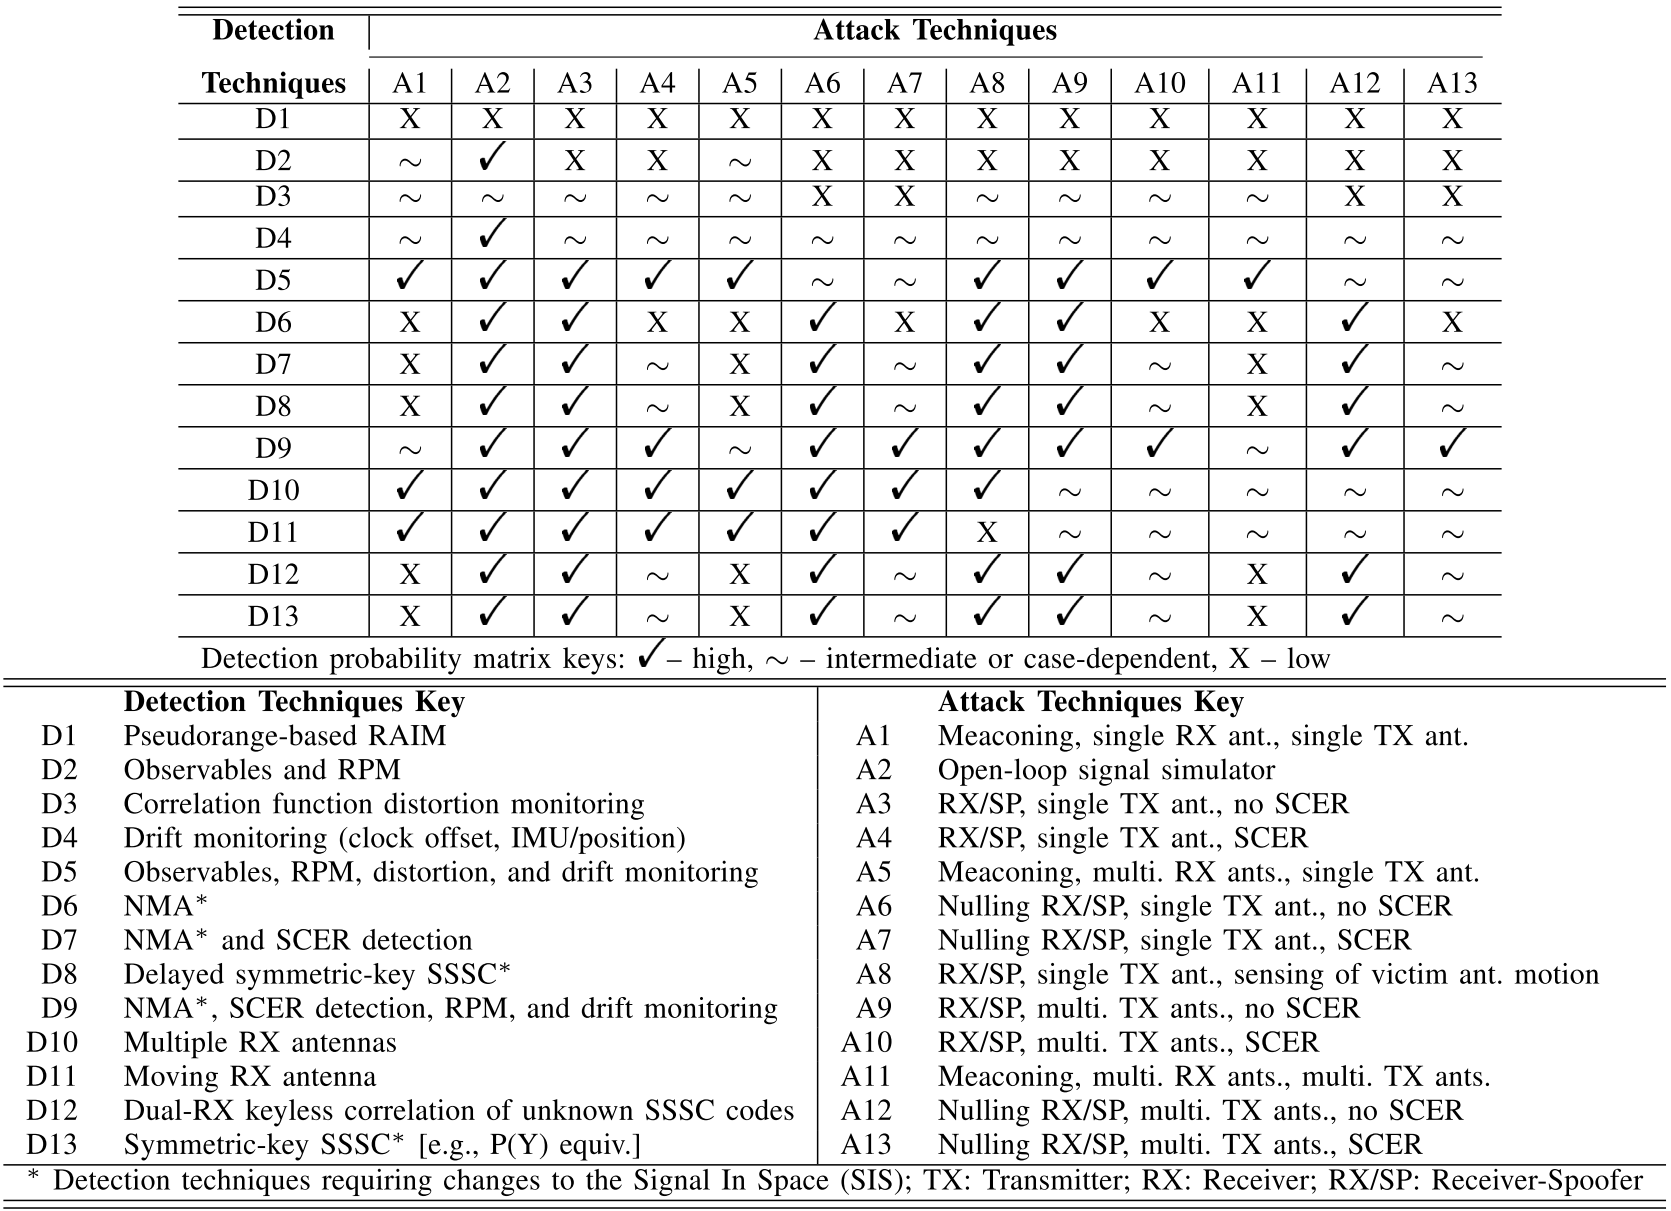
\includegraphics[width=14cm, keepaspectratio]{Figures/Attack and defence summary.png}
        \caption{Summary of spoofing attack and defence methods and their effectiveness against each other as found in \cite{RN12}}
    \label{fig:SpoofDefenceSumm}
    \end{centering}
\end{figure}

%
% Subsection - Anti-spoofing
%

\subsection{Anti-Spoofing Literature}
Within the literature there has been a categorisation of anti-spoofing techniques into detection and mitigation. Detection techniques have been more researched since they
are much easier to implement. Mitigation requires overcoming the spoofing attack and maintaining lock with the legitimate GPS signals. It is common within research to
investigate methods of spoofing attack and to combine this with recommendations for anti-spoofing. This was the case with \textcite{RN6}, \textcite{RN32},
\textcite{RN33} and \textcite{RN23}. The later, as mentioned above in Section \ref{Subsec:SpoofLit} a spoofing device was developed and tested against some anti-spoofing
methods. From this anti-spoofing recommendations were developed. The recommendations are as per \citeauthor{RN6}. \textcite{RN6} investigated antispoofing techniques
available. Antispoofing can be broken down into 2 groups spoof detection and spoof mitigation, with each of these being able to be further broken into subcategories. 

In \textcite{RN32} a review and analysis of the GNSS spoofing threat as well as the countermeasures of the time was provided. This report aimed
to fill the gap in 3 main areas of GNSS spoofing research, namely assessing the exact threat scenarios for commonly cited targets, investigate the practical impediments
of performing a spoofing attack in the field and lastly to survey and asses the performance of proposed GNSS spoofing defences. When defining spoofing, \citeauthor{RN32}
determined that a power ratio (spoofed vs authentic) of just 1.1 was sufficient to force the receiver to move onto the spoofed signal. And with authentic GNSS signal
strengths of approximately $-153dBW$ to $-160dBW$, this ratio is easy to achieve. It was noted that the
only detectable differences between a legitimate and spoofed one is the timing difference, signal angle of arrival, signal strength, Doppler shift and SNR. Most receivers
as of \citeyear{RN32} were not capable of registering these differences. The AGC (Automatic Gain Control) functionality common on GNSS receivers adjusts the signal gain
to compensate for any changes in the received signal strength, and in doing so makes the receiver more susceptible to a spoofing attack. The two main spoofing attack
types analysed were \emph{Meaconing} and \emph{SCER}. SCER is an evolution of the Meaconing attack where a single satellite signal is rebroadcast after a set delay.
Meaconing is the simplest spoofing attack and is a capture and re-transmission attack. This attack is difficult to perform on the military P(Y) code, but simple to perform
for the civilian C/A code. The most commonly referred to GNSS spoof attack targets came in the form of Power Disruption networks, shipping, aircraft, trains, criminal
security tags and mobile phones. Each of these examples were analysed in detail for potential attack vectors.
It was also noted that there are significant practical difficulties to performing a spoofing attack outside of an academic setting where variables can be tightly
controlled. First and foremost the cost of the hardware, while declining quickly, is still out of reach of many of the general public costing upwards of \$2300 at the
time. Current pricing for the USRP N210 in Australia is approximately \$4000. 
Those without the technical know how could purchase an off the shelf GNSS simulator unit, however these start at \$20,000 for a multi constellation generator. Practical
difficulties continue with distance from the target, which, due to the inverse square law of radio propagation means to ensure a sufficiently high SNR that distance from
attacker to target should be minimised. This is made difficult if the target is moving. Other difficulties were raised including need for direct line of sight and the need for
multiple simulators for multi GNSS receivers. 
While it was found that current generation GNSS receivers were susceptible to spoof attacks, there were countermeasures that could be employed to either detect or
mitigate the spoofing threat. Of the proposed GNSS spoofing countermeasures all can be summarised with four categories, Signal processing defences, cryptographic
defences, Correlation with other timing sources, Radio spectrum and antenna defences. It was found that at least 1 method from each of the categories was highly effective
at defending against an attack. Given the practical difficulties in performing a spoofing attack and the effective defences that have been developed (although not used in
the wider community as yet) it was concluded that the threat posed by GNSS spoofing was low but with the potential to increase as the practical implementation became
easier and cheaper and if companies did not implement countermeasures.
Recommended future work was based around real time detection and location of spoofing attacks.

The review provided in \cite{RN32} was expanded by a review in \citeyear{RN33} by \textcite{RN33}. \citeauthor{RN33} provided a survey of the spoofing and anti-spoofing
measures that have been researched recently. A detailed list of spoofing and anti-spoofing techniques were covered within the
literature, but as mentioned above all can fit within the 2 categories of forwarding or generating based techniques. From the research it was found that most of the
anti-spoofing techniques require some form of hardware alteration. There were some methods that did not require such modifications, namely those that relied upon antenna
array detection and angle of arrival detection methods. It was found that there is no spoofing method that is immune to all anti-spoofing techniques, and equally there
is not single anti-spoofing method that is able to detect and mitigate all spoofing methods. It was advised to continue researching and developing advanced anti-deception
systems since the deception models will continue to advance. 

The authors outlined challenges faced by GNSS systems which include: PVT accuracy, availability of GNSS systems, integrity of the system, and the ease in which
interference can occur. 

From \cite{RN12} the defence techniques could be broken down into three categories; pseudo-range RAIM (receiver autonomous integrity monitoring),
looking at the difference between a true and spoofed signal, and looking for interaction between true and spoofed signals. Pseudo-range RAIM is considered
too weak against modern spoofing attacks and was not considered in this publication. The specific methods of defence tested in this paper  
were advanced signal processing techniques, encryption based, drift monitoring, signal geometry and multi pronged spoofing defence.

The effectiveness of each spoof detection technique was tabulated and compared. As was the spoof mitigation techniques. Each detection and mitigation method was given a
complexity, effectiveness and spoofing scenario generality rating with notes made about the received capability requirements and are summarised in Table
\ref{tab:SpoofDetectSum} and Table \ref{tab:SpoofMitigateSum}. It was shown that with modest, low complexity spoof detection and mitigation strategies some of the spoof
attacks were able to be overcome.

\textcite{RN7} discussed a method of spoof detection by creating unique a fingerprint from each of the transmitting satellites. This fingerprint algorithm was able to determine if a transmission was
authentic or spoofed. This fingerprinting algorithm implementation was found to be fast, simple, cost effective and robust when compared to previous hardening attempts.

Another form of spoof detection was discussed in \cite{RN10}. \textcite{RN10} used multiple receivers in order to process the signals and determine if the signals were
authentic or spoofed. These techniques were varied and ranged from simple methods like monitoring the power level
of the received signal, to more complex like analysing the presence of vestigial peaks in the correlator output. When there is no spoofer present there will be unique signal
characteristics at each of the receivers. The concept of detecting a spoofing event was to compare the position of each receiver against the known relative positions. This
was chosen as it will not require any hardware modifications and the software processing can be done by an external processor, making it suitable for retrofitting to
existing systems. The testing was performed under the assumption that the spoofing transmitter only had one antenna. In the
first case there was approximately 1\% chance of a false alarm while the probability of detection was found to be intractable.
It was noted that to enable an initial statistical analysis of the solution, some simplifying assumptions were chosen. As such, future works should attempt to reduce the
simplifications where possible to create results that are applicable to real world scenarios.

Other means of spoofing detection aim to use existing infrastructure or existing sensors built into products. In \cite{RN1} \citeauthor{RN1} proposed a method of spoofing
detection and localisation using V2V (Vehicle to Vehicle) communications. Using a network of cooperative vehicles the spoofer could be localised by analysing the respective
Doppler shifts. After laboratory testing on stationary spoofers, it was found to be effective at providing an approximate location at up to 200m away.
When the spoofer was moving, this was decreased to 50m and was movement direction agnostic. In another paper, \citeauthor{RN24} proposed a method for detecting spoofing
attack on commercial airplanes by monitoring the broadcast information for erratic or unexplainable changes in position or velocity \cite{RN24}. This was named
Crowd-GPS-sec.

\textcite{RN31} and \textcite{RN42} discuss methods of spoofing detection on mobile devices.
The Android operating system released an update in 2016 the Android API which included access to the Raw GNSS properties including navigation messages, pseudo-ranges,
Doppler frequencies, constellation status and others. An overview of the changes made over recent versions can be found in \cite{RN39}. From these properties a GPS spoof detection program
was developed without the need to modify the hardware of the GPS receiver or the transmitting satellite. From the available information and sensors of the chosen phone, 4 sensor combinations were chosen 1) network location provider, 2) AGC (automation gain control) and C/No engine,
3) inertial sensor data and 4) pseudo-range residual metrics. It was noted that there exists an app that combines all of the mentioned methods together "GNSSAlarm" which was
used for testing. From testing it was found that phones tend to give a higher priority to GPS based location than that of other methods (network based). 
From testing it can be seen that each of the metrics available can be used to combat certain types of spoofing attacks, and when used together as in GNSSAlarm, 
a robust solution is available \cite{RN31}.

The existing cellular network infrastructure can be used to determine if position and time information received from GNSS sources is accurate. Previously
proposed methods for GPS signal detection have typically required special hardware and are difficult to deploy since they are based on the physical properties of the
received GPS signal. This new proposal uses broadcasts from cellular towers to validate the position received by the GPS signal. Parameters from the cell towers used to
determine the validity of the GPS signal include the number of in-range base stations, the distance to those stations and the received power of the signal. This method
was tested against a real spoofing attack and it was found that the there was 0\% false positive complete detection of the spoofing signals tested with negligible delay
\cite{RN42}.

As mentioned above, there has also been research performed in the context of spoof mitigation. There is a cross over between detection and mitigation since the presence of
a spoofer or spoofed signal must first be detected before it is acted upon.

The most up to date sources, \cite{RN34} \cite{RN36} \cite{RN18}, propose spoofing mitigation strategies that are reflective of the advancement of technology over the
past decade. \textcite{RN34} provided a detailed survey of the current GNSS interference landscape in relation to the aviation industry. The development of mitigation
techniques was based around the mathematical modelling of different attack types. A detailed summary of mitigation strategies
based on the attack/interference type was provided. By grouping all of the resources together this paper was able to produce a single repository where defences against
all attack categories mentioned above. Jamming and spoofing signal models were presented, with a class baseband signal model and a list of unknown parameters. Jammers
were classified into five different classes based on the complexity of the attack. Single/multi tone AM/FM type attacks made up class 1 jammers, single and multi chirp
attacks made up class 2 and 3. Chirp signals with frequency bursts were class 4 jammers and class 5 were DME-like/pulse jammer. Spoofers were divided into simplistic
spoofer, intermediate spoofer, sophisticated spoofer and meaconer. The unintentional interference models were also discussed and it was noted that adjacent channel
interference is typically harmonics leaking over from other frequency bands. This may be from DVB or LTE sources and is modelled as AM or FM tones. Co-channel
interference is most often caused by other GNSS services transmitting at the same frequency. This is modelled as increased AWGN (Additive White Gaussian Noise). A summary
of the different detection methods was produced. Detection of a single interference type is simple and can be determined using PDFs (probability density functions). The
scenario in which there is no interference will be Gaussian, whereas in the presence of interference the received signal may not be depending on the interference type.
Front end detection uses the raw signal before going though the ADC, commonly AGC detectors are used. Since the AGC will attempt to maintain a steady input power it can
be monitored to see if the gain requirement suddenly drops, indicating a high power signal and most likely a spoofer. The next type of detection method was the
pre-correlator type, in which the signal is converted to a different domain to estimate characteristics of the signal or separate the GNSS and interference signals. The
next type of mitigation strategies were post-correlator types. These are typically reserved for spoofing mitigation as opposed to jamming mitigation. This anti-spoofing
method is only effective if the authentic signal can be recognised and separated from the fraudulent one. If not then mitigation is not achievable. The final technique is
performing mitigation at a navigation level. This removes the requirement for adding special correlator hardware and uses the typical output from normal receivers. This
method works by discarding signals that are deemed to be counterfeit.

\textcite{RN36} provided an implementation of the Galileo OS-NMA for embedded devices running ARM based processors. The OS-NMA is an
attempt to include spoofing countermeasures within the message structure from the satellite. The
NMA cryptographic data is mostly unpredictable, which can be used to protect against replay attacks like meaconing attacks \cite{RN37}.
Software profiling was performed with performance comparisons undertaken
between different platforms. There are OSNMA ready commercial hardware receivers, however the authors decided that a software implementation would be best suited as new
features are easily added and the algorithm can be easily accessed and modified as needed. An overview of the OS-NMA was provided with parameters, values and
descriptions. Testing was performed on a Dell PC with Xeon processor and an ODroid running ARM based exynos processor. It was shown that the ARM based device suffered
with execution times ballooning. However the receiver was able to decode the OS-NMA code successfully. Future work will go into optimising the software for different
platforms and utilising more powerful hardware to close to gap with more powerful PC machines.

\textcite{RN18} developed an SDR for spoofing mitigation purposes since typical COTS GNSS receivers do not have a way of being upgraded since their hardware is set and
not able to change. Having a receiver with upgradeable hardware, such as that found in SDR platforms, would make for an ideal GPS receiver. As such SDRs are well suited
as GNSS receivers, however, they are challenged by processing the GNSS data and anti spoofing method. \citeauthor{RN18} performed experiments to see how effective SDR
platforms were at implementing a mitigation strategy in real time. A reduced complexity MMSE (minimum mean squared error) algorithm was developed for use on the in house
developed SDR platform. This algorithm was compared against MF (matched filter) techniques. It was found that at an ISR (interference to signal ratio) of 30dB that MF
correlators were unable to receive any usable signal, with BER (bit error rate) of approximately 50\%. Using the proposed maximise correlator, at a 30dB ISR, showed a BER
gain of approximately $10^5$. However, in testing it was found that most COTS receivers were not able to perform these duties in real time due to the increase in
complexity of the antispoofing algorithms.

A consistent theme in the literature is the inclusion of cryptography into GNSS constellations. The method employed by \citeauthor{RN13} included adding digital signatures within the GPS civil navigation message. This type of cryptographic defence
will secure the receiver against replay spoof attacks. Authentication of each civil GPS signal is performed every 5 minutes.
For the proposed authentication strategy a $P_D$ of >0.97 was achieved over the range of $37$-$51 dB-Hz$.
The implementation of such a system would require modifications to the GPS satellite system themselves, as well as a redesign of GPS receivers.
The modifications required for the GPS receivers were documented in detail in \cite{RN13}. For systems that can not easily or readily upgraded to
take advantage of these improvements an external device called "The GPS Assimilator", as proposed in \cite{RN19}, could be used to clean the incoming
signals.
Although it was noted that receivers based on SDR platforms would be able to implement the authentication algorithm easily. 

The summary of spoofing at the time of \cite{RN11} is shown in Table \ref{tab:GPSMitigationSum}. While there are more complicated strategies available now, many
commercial receivers do not implement them, as such the basic strategies are still valid.

\renewcommand{\arraystretch}{1.2}
\begin{table}[!h]
    \begin{center}
        \caption{Summary of Spoofing Mitigation Methods from \cite{RN11}}
        \label{tab:GPSMitigationSum}
            \begin{tabular}{ m{3cm} | m{5cm} | m{5cm} }
                \hline
                \textbf{Test Statistic} & \textbf{Function} & \textbf{Limitation} \\
                \hline
                Absolute signal power & Limit the spoof signal power & Antenna attitude and environment related \\
                Signal power changing rate & Detect stationary spoof station & Antenna attitude and environment related \\
                Relative signal strengths on all carriers & Detect spoofing on single carrier & Affected by ionosphere refraction \\
                Range rate & Bound the phase and code range rate & Relate to GPS receiver's moving direction \\
                Doppler shift & Detect spoof that uses one transmitter to spoof all satellites & None \\
                Correlation peaks & Correlate L1/L2 binary messages & Low performance on Y-code \\
                GPS signal after removing all navigation data & Recover authentic data & Requires low spoof/authentic signal power ratio \\
                Range differences: phase/code, L1/L2 & Identify signal source & Needs to be L1/L2 receiver \\
                Ephemeris data & Verify ephemeris data including satellite position & None \\
                Signal power and data & Jump detection & None \\
                \hline
            \end{tabular}
    \end{center}
\end{table}
\renewcommand{\arraystretch}{1}


\renewcommand{\arraystretch}{1.2}
\begin{table}[!ht]
    \begin{center}
        \caption{Summary of Spoofing Detection Methods from \cite{RN6}}
        \label{tab:SpoofDetectSum}
        \makebox[1 \textwidth][c]{
        \resizebox{1.1 \textwidth}{!} {
            \begin{tabular}{ m{40mm}|m{35mm}|c|c|m{30mm}|m{20mm} }
                \hline
                \textbf{Anti-Spoofing method} & \textbf{Spoofing Feature} & \textbf{Complexity} & \textbf{Effectiveness} &
                \textbf{Receiver required capability} & \textbf{Spoofing scenario generality} \\
                \hline
                $C/N_0$ monitoring & Higher $C/N_0$ & Low & Medium & $C/N_0$ monitoring & Medium \\
                Absolute power monitoring & Higher amplitude & Low & Medium & Absolute power monitoring & High \\
                Power variation versus receiver movement & Higher power variations due to proximity & Low & Low & Antenna movement/ $C/N_0$ monitoring & Low \\
                L1/L2 power comparison & No L2 signal for spoofer & Medium & Low & L2 reception capability & Low \\
                Direction of arrival comparison & Spoofing signals coming from the same direction & High & High & Multiple receiver antennas & High \\              
                Pairwise correlation in synthetic array & Spoofing signals coming from the same direction & Low & High & Measuring correlation coefficient & High \\
                TOA discrimination & Inevitable delay of spoofing signal & Medium & Medium & TOA analysis & Low \\
                Signal quality monitoring & Deviated shape of authentic correlation peak & Medium & Medium & Multiple correlators & Low \\
                Distribution analysis of the correlator output & Perturbed amplitude distribution due to spoofing-authentic interaction & Low & Medium & Distribution
                analysis of correlator outputs & Medium \\
                Consistency check with other solutions & Inconsistency of spoofing solution & High & High & Different navigation sensors & High \\
                Cryptographic authentication & Not authenticated & High & High & Authentication & High \\
                Code and phase rate consistency check & Mismatch between artificial code and phase rate & Low & Low & - & Low \\
                GPS clock consistency check & Spoofing/authentic clock inconsistency & Low & Medium & - & Medium \\ 
                \hline
            \end{tabular}
        }
        }
    \end{center}
\end{table}
\renewcommand{\arraystretch}{1}

\renewcommand{\arraystretch}{1.2}
\begin{table}[!ht]
    \begin{center}
        \caption{Summary of Spoofing Mitigation Methods from \cite{RN6}}
        \label{tab:SpoofMitigateSum}
        \makebox[1 \textwidth][c]{
        \resizebox{1.1 \textwidth}{!} {
            \begin{tabular}{ m{40mm}|m{35mm}|c|c|m{30mm}|m{20mm} }
                \hline
                \textbf{Anti-Spoofing method} & \textbf{Spoofing Feature} & \textbf{Complexity} & \textbf{Effectiveness} &
                \textbf{Receiver required capability} & \textbf{Spoofing scenario generality} \\
                \hline
                Vestigial signal detection & The authentic signal is still present and can be detected & High & Medium & Multiple receive channels & Medium \\ 
                Multi-antenna null steering & Spoofing signals coming from same direction & Medium & High & Multiple receive antennas & High \\
                RAIM & Higher residuals for spoofed measurements & Medium & Medium & - & Medium \\
                \hline
            \end{tabular}
            }
            }
    \end{center}
\end{table}
\renewcommand{\arraystretch}{1}

%----------------------------------------------------------------------------------------
%	SECTION 3
%----------------------------------------------------------------------------------------

\section{Literature Review Conclusion}
Some of the early assessments of the spoofing threat included methods for performing said attacks using specialised hardware \cite{RN23}. This increased the technical
knowledge required to be able to perform an attack.

Common recommendations from the literature was the implementation of, at a minimum, basic anti-spoofing infrastructure. This is more common place in applications that
have suitable software processing capabilities. But dedicated COTS receivers do not typically have any defence strategies in place.
Cryptographic solutions are frequently suggested in literature, and have been implemented with success. However such implementations require alterations to the space
segment of the GNSS constellation. This may be implemented for the next generation satellites but for now this is not feasible. 

Some literate have proposed workarounds should the constellations be upgraded, such as \cite{RN19} where an external device performs the cryptographic checks before
passing the signal to the outdated receiver.

Areas of future research were also outlined and include but are not limited to interconnecting the satellites together, increasing accuracy of
atomic time keeping as well as introducing advanced anti-spoofing techniques, more wide spread support of multi constellation receivers, and increasing anti interference
capabilities of receivers through either hardware, software or both \cite{RN33}.

Anti-spoofing methods have previously been abandoned because of cost and complexity issues \cite{RN7}.